\documentclass[12pt, a4paper,reqno]{article}

\usepackage{amsmath}
\usepackage{amssymb}
\usepackage{graphicx}
\usepackage{float}
\usepackage{caption}
\usepackage{subcaption}
\usepackage{pdfpages}
\usepackage{minted}
\usepackage{color, soul}

\setlength{\parindent}{0pt}
\setlength{\parskip}{1em}

\DeclareMathOperator*{\argmin}{argmin}


%
% Begin Document
%
\begin{document}

% TODO: Add date
% Cover Page

\includepdf[pages=-]{End_Assessment_Front_Page_HYXC3.pdf}


%
% Question 1
%
\section*{Question 1}

% Subsection 1(a)
\subsection*{1(a)}
With reference to the diagram of the basic \emph{logistic unit} on the following page:

The input vector $\mathbf{x}$ is the input to the \emph{logistic unit}.

Each input ${x}_i$ has an associated weight $\theta_i$. The weights are set to a random value prior to \emph{training}. The \emph{training} process determines these weights.

The product of each input $x_i$ and weight $\theta_i$ is summed to produce a weighted sum $z$.

The output, $h_\theta(x)$, is the the non-linear \emph{activation function}, $h$, applied to $z$.

% Subsection 1(b)
\subsection*{1(b)}

Consider the diagram of Question 1(a).

The weighted sum of the inputs, $z$, is:

\begin{equation}
z = \sum_{j=1}^{n}\theta_j x_j = \theta^T x
\end{equation}

where $x_i$ is the $i^{th}$ element of input vector $\mathbf{x}$ of length $n$, and $\theta_i$ is the associated \emph{weight}. 

And, the output from the \emph{logistic unit}, $h_\theta(x)$, is:

\begin{equation}
h_\theta(x) = h(z)
\end{equation}

where $h$ is a non-linear \emph{activation function}.

% Subsection 1(a) - diagram
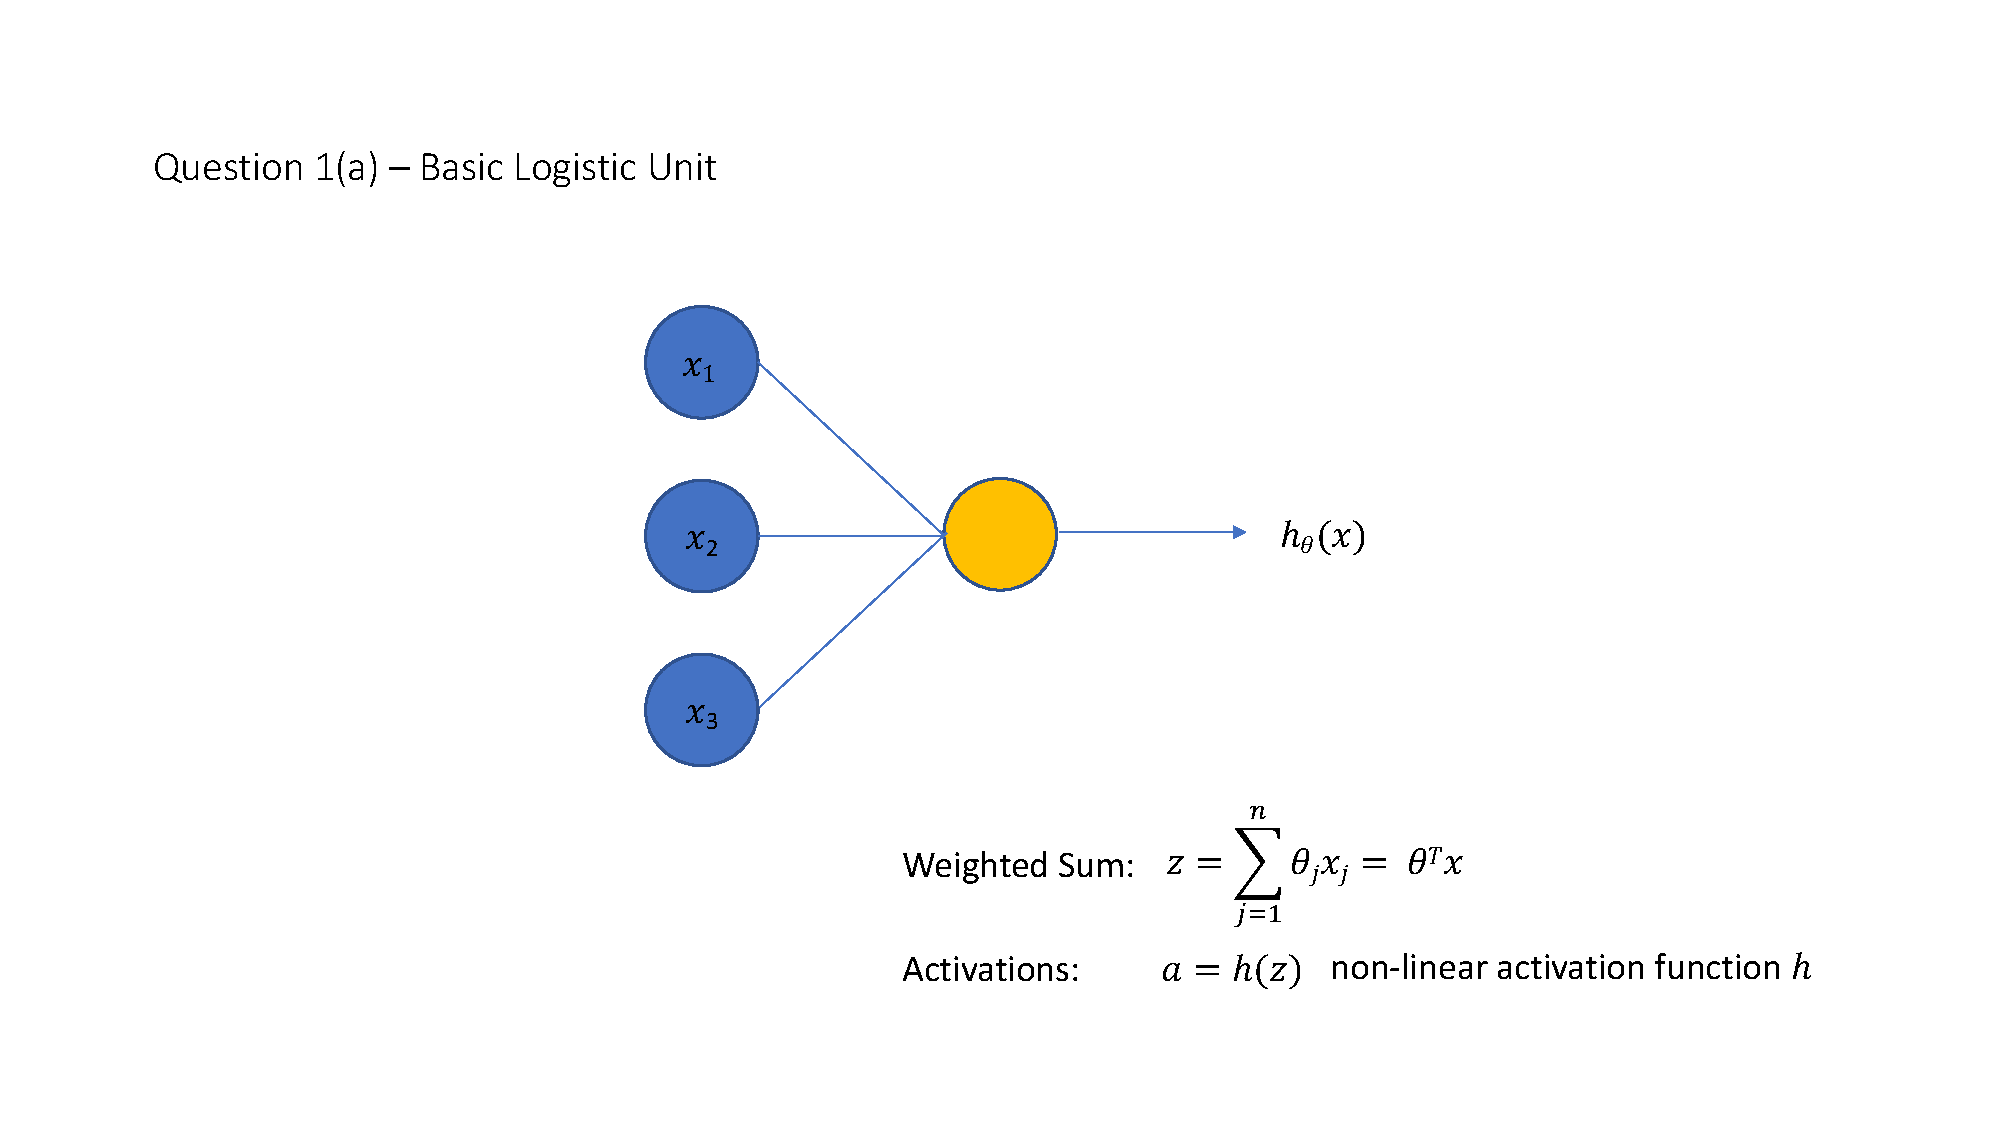
\includepdf[angle=+90]{question_1a.pdf}

% Subsection 1(c)
\subsection*{1(c)}
See diagram on following page.

% Subsection 1(d)
\subsection*{1(d)}
Consider the diagram of Question 1(c).

Firstly, consider the data transformation from the input vector $\mathbf{x}$ to the hidden layer. We now need two indices, one for the input vector elements, and one for the \emph{hidden layer} nodes. We will use $i$ for the input vector index, and $j$ for the \emph{hidden layer} nodes.

The weighted sum of the inputs at the $j^{th}$ \emph{hidden layer} node is:

\begin{equation}
z_j = \sum_{i=1}^{n}\theta_{ij} x_i
\end{equation}

where $\theta_{ij}$ is the weight between input element $i$ and \emph{hidden layer} node $j$, and $n$ is the length of the input vector $\mathbf{x}$.

Secondly, the output from each \emph{hidden layer} node is the non-linear \emph{activation function}, $h$, applied to each $z_j$:

\begin{equation}
h_{\theta j}(x) = h(z_j)
\end{equation}

 And finally, the output from the whole network, $h_\Theta(x)$ is the sum of the \emph{hidden layer} outputs:
 
\begin{equation}
h_\Theta(x) = \sum_{j=1}^{m}h_{\theta j}(x)
\end{equation}

where $m$ is the number of \emph{hidden layer} nodes.

% Subsection 1(c) - diagram
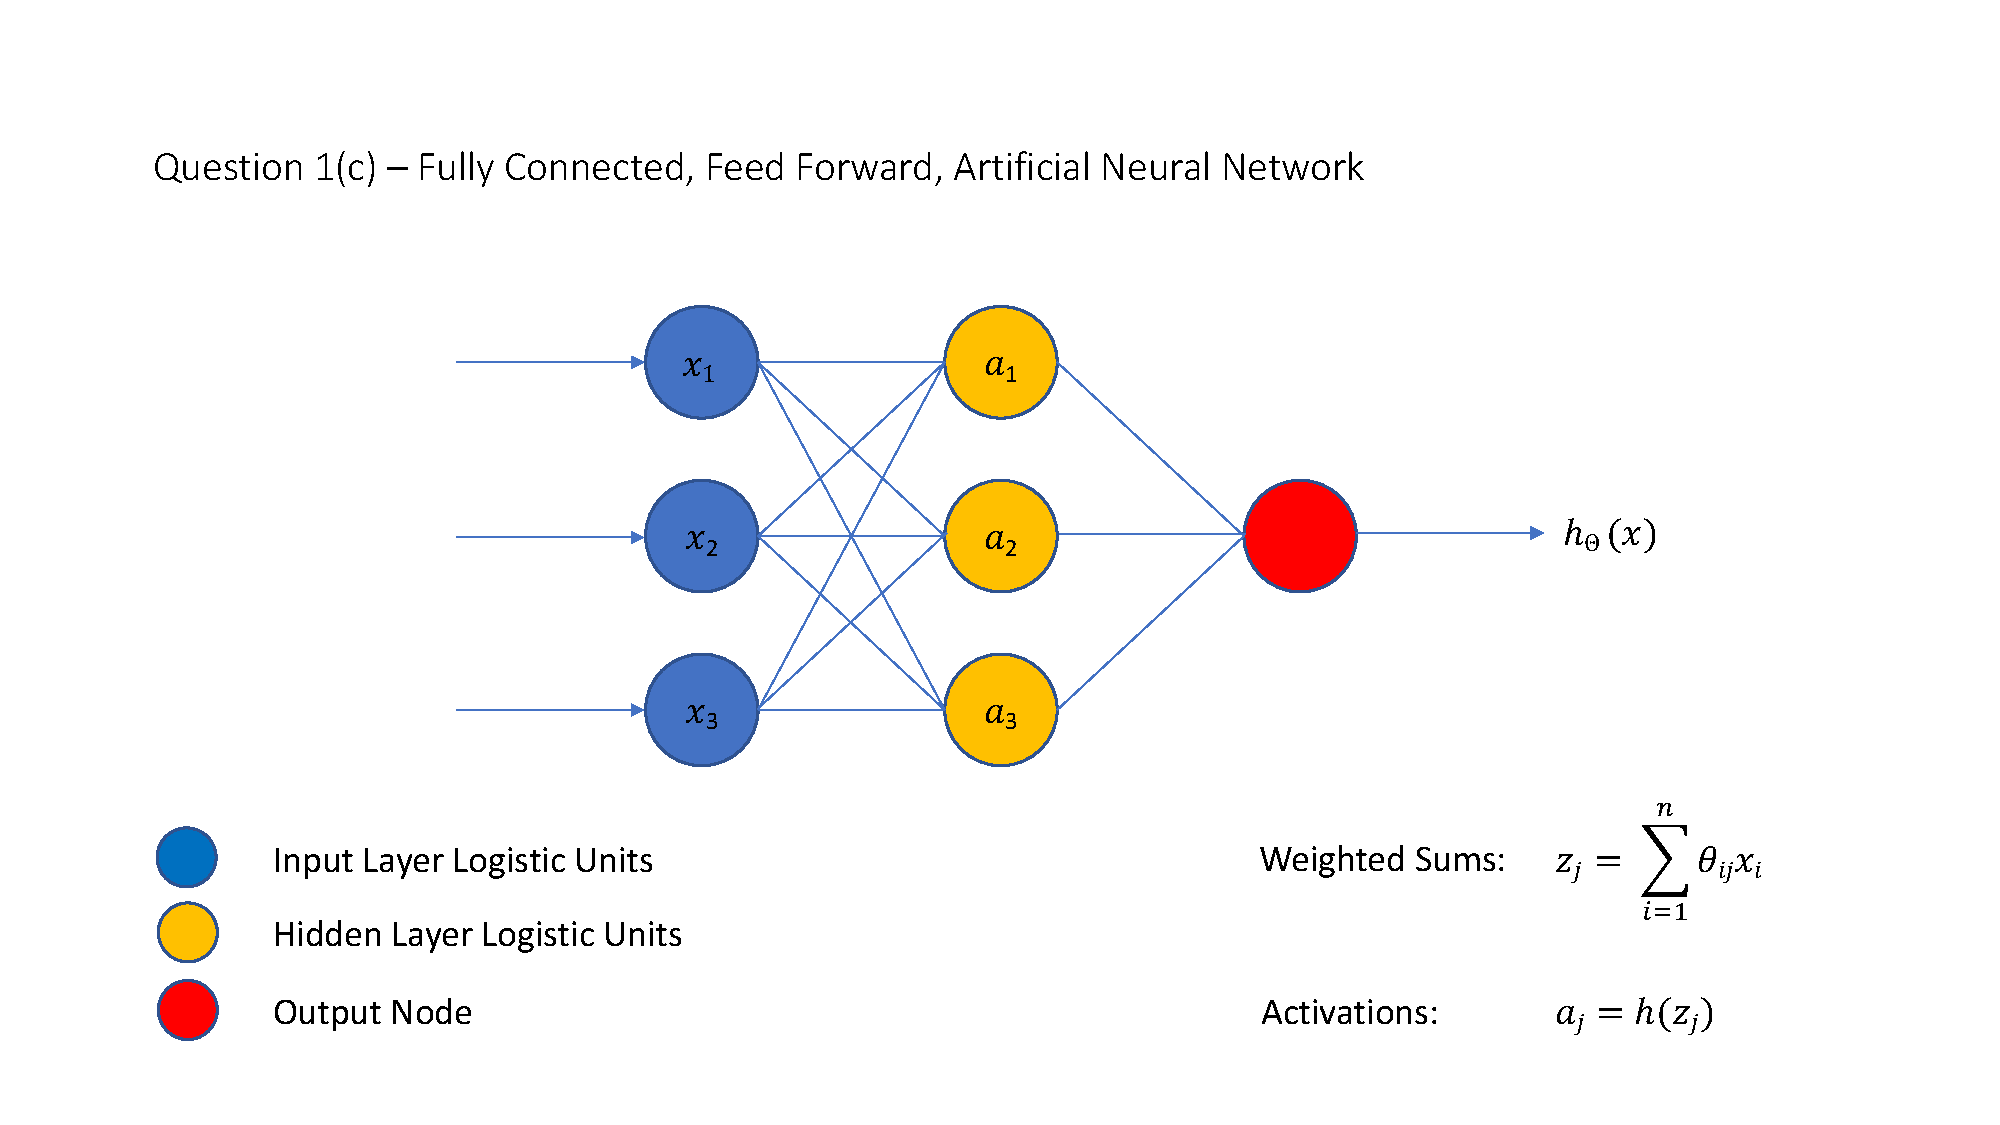
\includepdf[angle=+90]{question_1c.pdf}

% Subsection 1(e)
\subsection*{1(e)}

The cost function typically used to train neural networks for regression problems is \emph{mean square error}:

\begin{equation}
MSE(\Theta) = \frac{1}{m}\sum_{i}\sum_{j}(p_j^{(i)} - y_j^{(i)})^2
\end{equation}

The cost function typically used to train neural networks for classification problems is \emph{cross-entropy}:

\begin{equation}
C(\Theta) = -\frac{1}{m}\sum_{i}\sum_{j}y_j^{(i)}\log(p_j^{(i)})
\end{equation}

% Subsection 1(f)
\subsection*{1(f)}
Artificial Neural Networks (ANNs) are described as \emph{shallow} or \emph{deep}, and \emph{wide} or \emph{narrow}. \emph{shallow} or \emph{deep} refers to the number of layers in the network, and \emph{wide} or \emph{narrow} refers to the number of nodes in each layer.

The \emph{credit assignment path}, the CAP, of a neural network is a measure of the number of data transformations that occur as data passes through the network. For \emph{feed-forward} networks the CAP is the number of \emph{hidden layers} plus one.

A \emph{deep} neural network is generally considered to be a network with multiple layers and a CAP $>$ 2.

% Subsection 1(g)
\subsection*{1(g)}
The \emph{universal approximation theorem} states that, with appropriate parameters, single hidden layer feed-forward neural networks are \emph{universal approximators}. This means they can represent any continuous function. However, this requires an exponentially larger number of hidden layer nodes. And, training will not necessarily determine the parameters.

Deep networks provide a powerful representational framework because they have the potential to be \emph{universal approximators}, but with a limited width of hidden nodes. This makes the implementation of \emph{universal approximators} more feasible.


%
% Question 2
%
\clearpage\section*{Question 2}

% Subsection 2(a)
\subsection*{2(a)}

\emph{Gradient Descent} algorithms attempt to find the parameters $\theta$ which minimise the cost function $C(\theta)$ over the \emph{training set} using an iterative process:

\begin{equation}
\theta^{i+1} = \theta^i - \alpha\nabla_\theta C(\theta)
\end{equation}

where $\alpha$ is the \emph{learning rate}.

\emph{Batch Gradient Descent} uses the entire \emph{training set} at each iteration to calculate the gradient partial derivatives, $\nabla_\theta C(\theta)$. This produces accurate values for the partial derivatives, but is potentially slow for large \emph{training sets}.

\emph{Stochastic Gradient Descent} uses a random sub-set of the \emph{training set} at each iteration to calculate the gradient partial derivatives, $\nabla_\theta C(\theta)$. This is faster than \emph{Batch Gradient Descent}, but can produce erratic values for the partial derivatives. 

For \emph{convex} cost functions \emph{Batch Gradient Descent} will always converge to the \emph{local minima} which is also the \emph{global minima}. This is not the case for \emph{non-convex} cost functions, where \emph{local minima} are not necessarily \emph{global minima}. A bad choice of $\theta^0$ may result in \emph{Batch Gradient Descent} getting ``stuck" in a \emph{local minima}. Because the gradient partial derivatives of \emph{Stochastic Gradient Descent} are erratic, this provides a mechanism of ``jumping out of" a \emph{local minima} and improves the probability of finding the \emph{global minima}.

% Subsection 2(b)
\subsection*{2(b)}

When attempting to find the minimum of a cost function using \emph{Stochastic Gradient Descent}, the iterative process ``jumps'' around the minimum, and it is difficult to determine when a minimum has been reached. For this reason alternative optimisation algorithms are typically considered for training.

% Subsection 2(c)
\subsection*{2(c)}
Consider the iterative minimisation process: 

\begin{equation}
\theta^{i+1} = \theta^i - \alpha\nabla_\theta C(\theta)
\end{equation}

where $\alpha$ is the \emph{learning rate}.

At each step the process ``advances" towards the minimum by the step size $- \alpha\nabla_\theta C(\theta)$, which uses the \emph{current} gradient.

The \emph{Momentum Optimisation} algorithm introduces the idea of including \emph{previous} gradients into the step size.  At each step the \emph{current} gradient is summed into a momentum term $m$, which includes \emph{previous} gradients (remember we use the negative gradient):

\begin{equation}
m^{i+1} = \beta m^i - \alpha\nabla_\theta C(\theta)
\end{equation}

The $\beta$ parameter is used to prevent the momentum getting too large, and is set between 0 and 1, typically 0.9.

The momentum $m$ is then used to update $\theta$:

\begin{equation}
\theta^{i+1} = \theta^i + m
\end{equation}

The result is that we now have an \emph{acceleration} towards the minimum.

This algorithm may result in an overshoot and oscillation before stabilising at the minimum.  

% Subsection 2(d)
\subsection*{2(d)}

Consider the momentum update equation of the \emph{Momentum Optimisation} algorithm:

\begin{equation}
m^{i+1} = \beta m^i - \alpha\nabla_\theta C(\theta)
\end{equation}

This uses the gradient at the current value of $\theta$.

However, the momentum $m$ is pointing in the general direction of the cost function minimum, so it makes sense to use a point further along in this direction, $\theta + \beta m^i$, to calculate the gradient, as this will be already closer to the minimum:

\begin{equation}
m^{i+1} = \beta m^i - \alpha\nabla_\theta C(\theta + \beta m^i)
\end{equation}
 
This is called the \emph{Nesterov Accelerated Gradient} algorithm.
 
$\theta$ is updated as per the \emph{Momentum Optimisation}  algorithm:
   
\begin{equation}
\theta^{i+1} = \theta^i + m
\end{equation}

The \emph{Nesterov Accelerated Gradient} algorithm is an enhancement to the \emph{Momentum Optimisation} algorithm, which can result in a significant increase in speed, and can reduce the overshoot and oscillations previously mentioned. 

% Subsection 2(e)
\subsection*{2(e)}

For optimisation problems where the \emph{objective function} has circular contours the negative gradient always points towards the \emph{objective function} minimum. This means that for an iterative process such as \emph{Gradient Descent} the steps are always in the direction of the minimum. This produces swift convergence to the minimum.

For an elongated \emph{objective function}, with steep sides, a narrow valley, and a bend in the valley, the negative gradient will not point towards the \emph{objective function} minimum if the current value of $\theta$ is at the opposite end of the valley. Large steps will be taken offset from the minimum direction. This will reduce the convergence rate. And where the negative gradient is the steepest is where the largest offset steps will be taken. This phenomena is observed for \emph{objective functions} with non-circular contours. 

The \emph{AdaGrad} algorithm addresses this problem by reducing the learning rate where the negative gradient is steepest. This reduces the step size away from the minima. Where the negative gradient is less steep the \emph{learning rate} is reduced by a lesser amount, preserving the step size towards the minimum. This is achieved by introducing a gradient squared term.

The \emph{AdaGrad} algorithm uses what is called an \emph{adaptive learning rate}. An advantage of this during \emph{training} is that less tuning of the learning rate $\alpha$ is required, as this is now ``self-tuning".

There is a problem though that the \emph{learning rate} may be reduced too much, and the minimisation of the \emph{cost function} comes to a stop prior to reaching the minimum. This is the reason why \emph{AdaGrad} is not generally used to train deep \emph{neural networks}.
 
% Subsection 2(f)
\subsection*{2(f)}

As previously stated, a problem with the \emph{AdaGrad} algorithm is that the \emph{learning rate} may be reduced too much, and the minimisation of the \emph{cost function} comes to a stop prior to reaching the minimum.

The \emph{RMSProp} algorithm address this problem by adding an exponential decay to the gradients. This means that only the most recent gradients are used in the minimisation process, and not all of the gradients.

\emph{RMSProp} performs better than \emph{AdaGrad} in most \emph{training} scenarios.

% Subsection 2(g)
\subsection*{2(g)}

The \emph{Adam} optimisation algorithm, \emph{adaptive moment estimation}, combines the following ideas from previously discussed algorithms.

From \emph{momentum} optimisation, \emph{Adam} borrows the idea of an exponential decay of previous gradients.

And from \emph{RMSProp}, \emph{Adam} borrows the idea of an exponential decay of previous gradients squared.

Because of its performance, \emph{Adam} is a standard algorithm for training deep neural networks.

% Subsection 2(h)
\subsection*{2(h)}

With reference to the diagram of \emph{Dropout Regularisation} on the following page.

Deep neural networks can be prone to overfitting. \emph{Regularisation} is a method of avoiding overfitting, and \emph{Dropout Regularisation} is one such method.

In \emph{Dropout Regularisation}, at every \emph{training} iteration every node, including the input nodes but excluding the output nodes, has a probability $p$ of being \emph{dropped}. When \emph{dropped} the output from the node is zero. The \emph{dropout rate} $p$ is typically 10\% to 50\%. On completion of training no nodes are \emph{dropped}.

Surprisingly, this method works, even though it would appear that useful information is being destroyed/ignored!

One way of looking at it is that the remaining nodes (the nodes that haven't been \emph{dropped}) have to work harder. And somehow have an enhanced memory or functional ability after training. The reliance on neighbouring nodes is reduced, and each node has to be more effective.

There is one factor that needs to be considered when moving from \emph{training} to \emph{testing}. During \emph{training}, with a \emph{dropout rate} of 50\%, say. There will be approximately 50\% less inputs nodes. Therefore during \emph{testing}, when no nodes are dropped, the input signal will be twice as strong. To account for this, each node's input weights are factored by $1 - p$. 

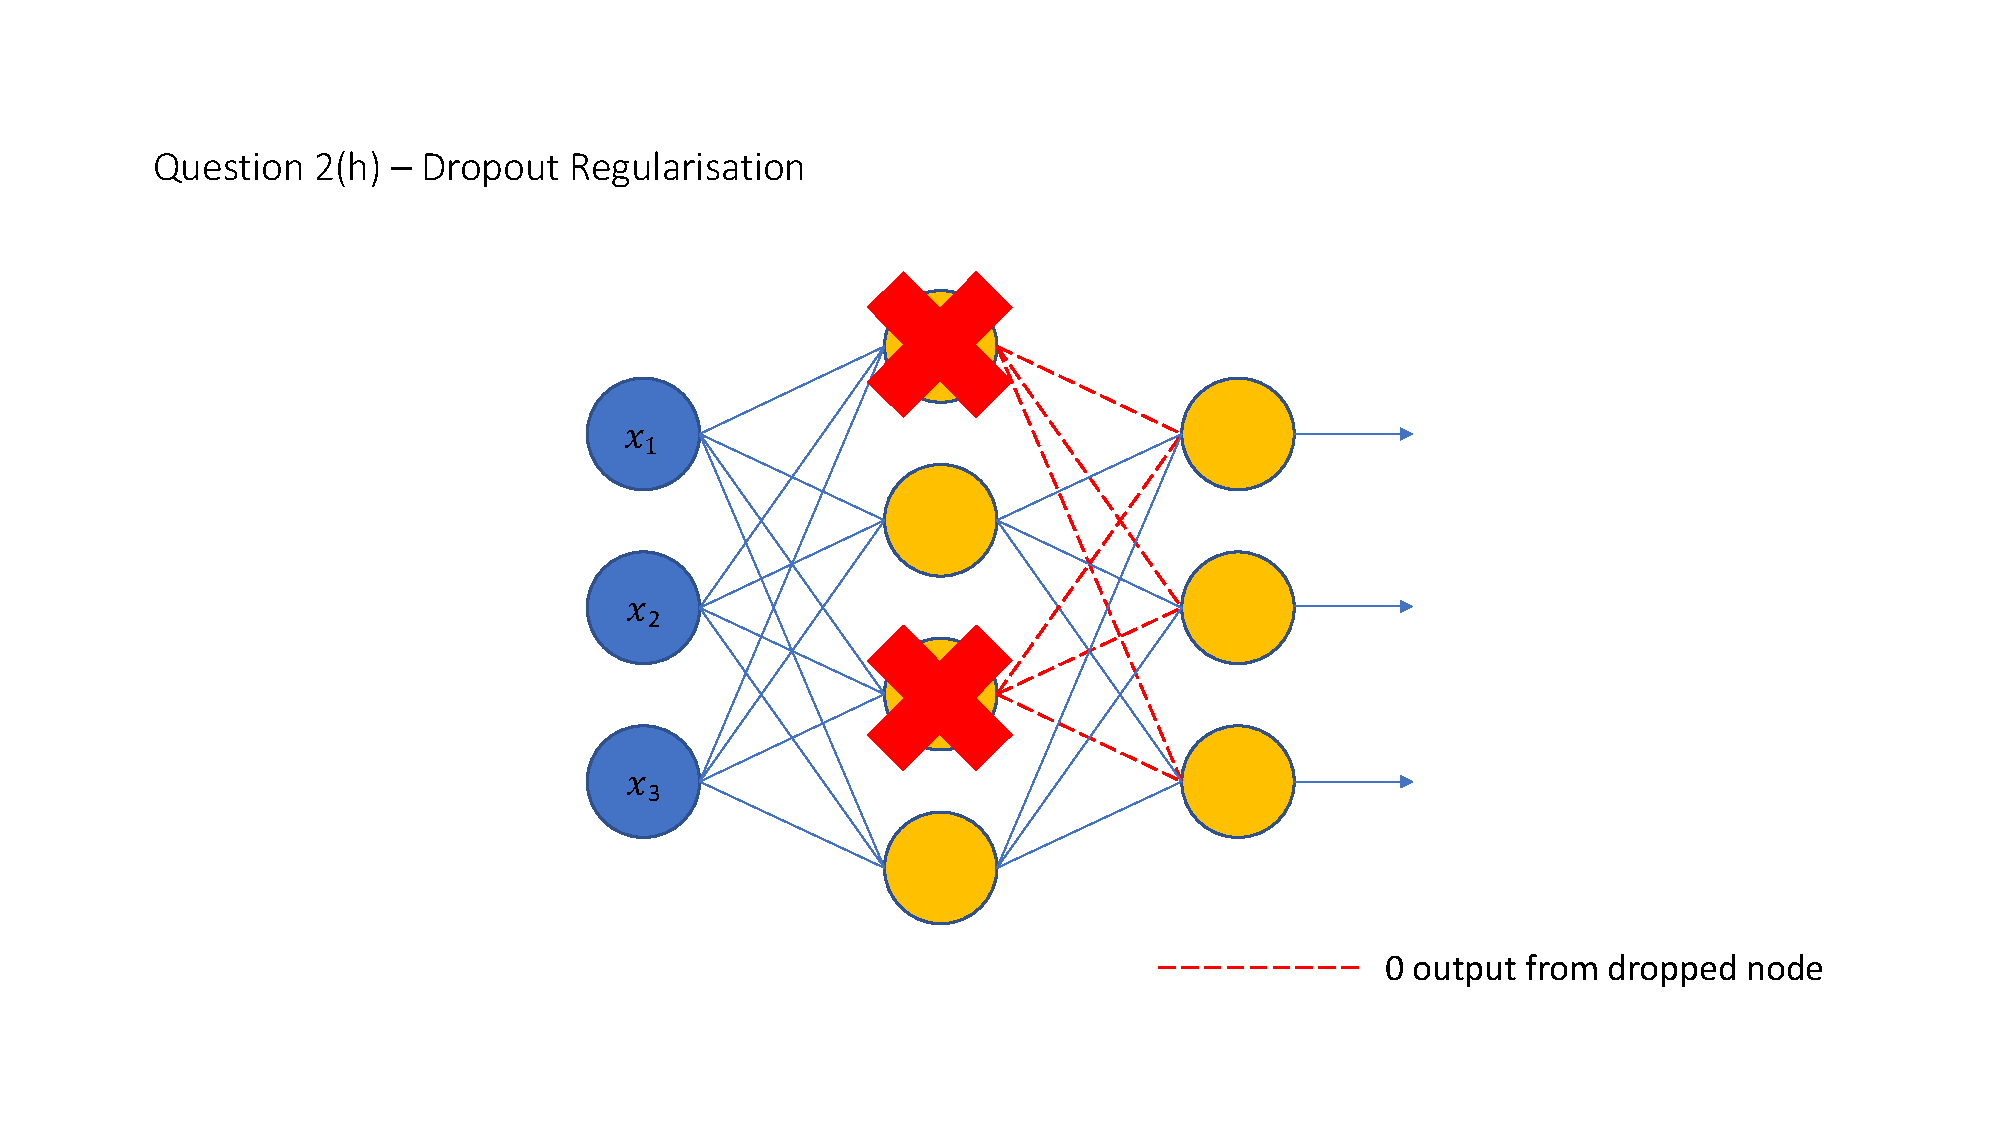
\includepdf[angle=+90]{question_2h.pdf}


%
% Question 3
%
\clearpage\section*{Question 3}

% Subsection 3(a)
\subsection*{3(a)}
The \emph{knowledge} based approach to \emph{artificial intelligence} is the encoding of knowledge as rules, and the subsequent use of logistical inference to make deductions from these rules.

One problem with this approach is that it is difficult to encode all knowledge as rules, for example intuition is difficult to encode as a rule.

Another problem is that the rules need to be added/amended/removed as the knowledge base changes.

% Subsection 3(b)
\subsection*{3(b)}

The \emph{machine learning} approach to \emph{artificial intelligence} is to enable a machine to \emph{learn} from data.

In this approach a machine is not given a set of rules. Instead, a machine is \emph{trained} on data from which patterns and relationships in the data emerge.     

This approach is more flexible than the \emph{knowledge} based approach.

% Subsection 3(c)
\subsection*{3(c)}

\emph{Features} are the elements of data which are relevant to a \emph{machine learning} task.

The \emph{machine learning} approach of \emph{feature engineering} ensures the appropriate \emph{features} are used for a \emph{machine learning} task. This consists \emph{feature selection} and \emph{feature extraction}.

\emph{Feature selection} is simply selecting the most appropriate features.

\emph{Feature extraction} is the generation of new features from existing ones. For example, creating a new feature $x^2$ from the exisiting feature $x$ may make a data set \emph{linearly separable} when the original data set was not. 

% Subsection 3(d)
\subsection*{3(d)}

Given \emph{training} data with associated \emph{labels}, e.g. this image (data) is an elephant (\emph{label}), \emph{Supervised Learning} predicts new outputs from new inputs. 

\emph{Unsupervised Learning} is the determining of relationships within unlabelled data, e.g. the clustering of data.

\emph{Reinforcement Learning} is the learning of a best action based upon being \emph{rewarded} for choosing the best action.

% Subsection 3(e)
\subsection*{3(e)}

In \emph{supervised learning}, a \emph{regression} problem is one which requires the output to be a numerical value, e.g. a share price.

In \emph{supervised learning}, a \emph{classification} problem is one which requires the output to be a \emph{class label}, e.g. this image of a digit is of the number (\emph{class}) 9.

% Subsection 3(f)
\subsection*{3(f)}
\hl{TODO}


%
% Question 4
%
\clearpage\section*{Question 4}

% Subsection 4(a)
\subsection*{4(a)}
\hl{TODO}

% Subsection 4(b)
\subsection*{4(b)}
\hl{TODO}

% Subsection 4(c)
\subsection*{4(c)}
\hl{TODO}

% Subsection 4(d)
\subsection*{4(d)}
\hl{TODO}

% Subsection 4(e)
\subsection*{4(e)}
\hl{TODO}

% Subsection 4(f)
\subsection*{4(f)}
\hl{TODO}

\begin{listing}
\inputminted[linenos]{python}{question_4f.py}
\caption{Question 4f}
\end{listing}

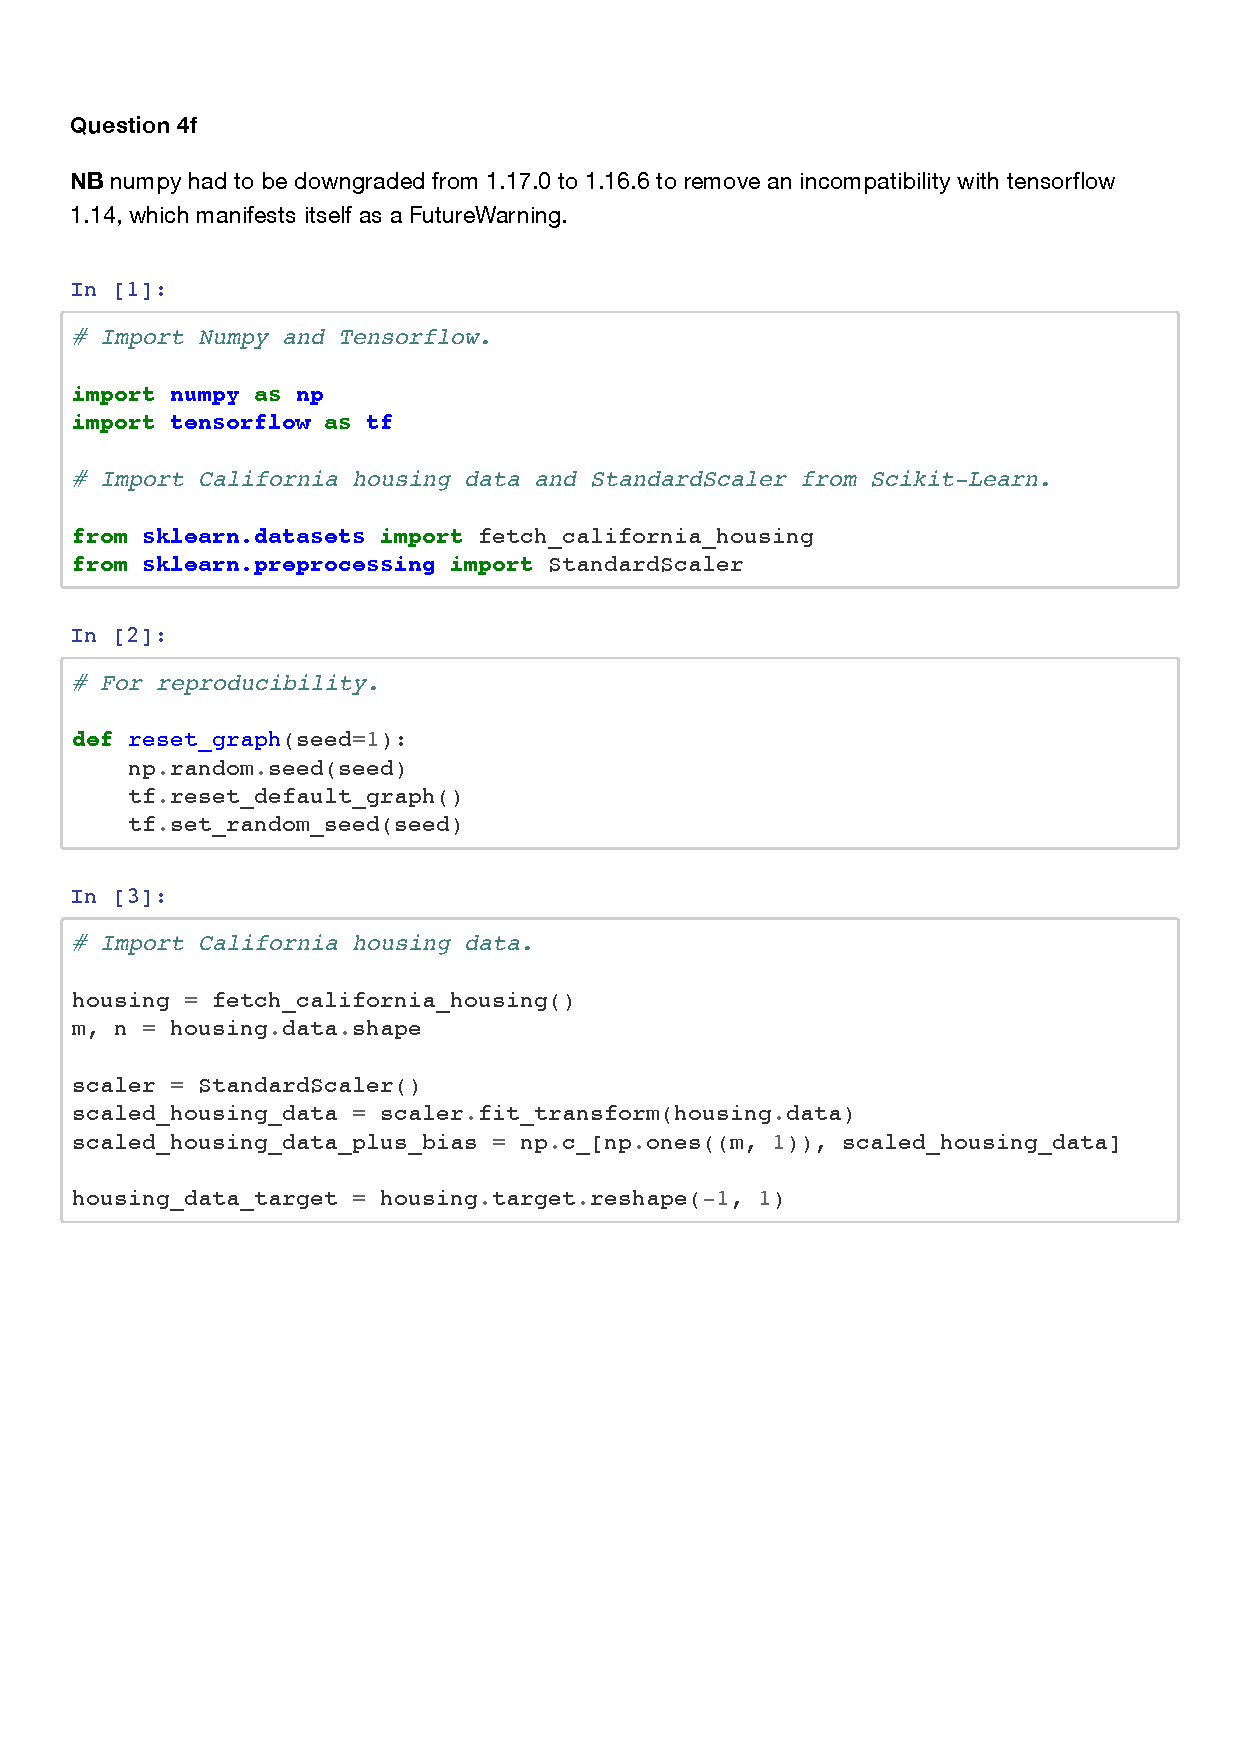
\includepdf[pages=-]{question_4f.pdf}

%
% Question 5
%
\clearpage\section*{Question 5}

% Subsection 5(a)
\subsection*{5(a)}

Data sets can have many features, sometimes too many. \emph{Dimensionality reduction} is the process of reducing the dimensions to a manageable size. \emph{Principal Component Analysis}, PCA, is a method to perform \emph{dimensionality reduction}.

PCA uses the idea that the dimensions with the most variance hold the most information.

PCA finds the axis in the data set with the most variance. This is called the first \emph{Principle Component, PC}. PCA then finds subsequent PCs orthogonal to previous ones containing the remaining variance, as many as there are dimensions. This is done using Singular Value Decomposition (SVD) of the co-variance of the data set. To then reduce the data set to $n$ dimensions, the data set is projected on to the hyperplane defined by $n$ PCs.

% Subsection 5(b)
\subsection*{5(b)}

The \emph{Explained Variance Ratio} is the proportion of the variance accounted for in each PC. 

% Subsection 5(c)
\subsection*{5(c)}

The \emph{kernel trick} is the observation that a valid (\emph{Mercer Theorem}) \emph{kernel function} $\mathcal{K}(x_i, x_j)$ is capable of finding the dot product of $\phi(x_i)$ and $\phi(x_j)$ without having to evaluate $\phi(x_i)$ or $\phi(x_j)$. This \emph{trick} enables \emph{Support Vector Machines} to efficiently classify non-linear data.

Similarly, \emph{Kernel PCA}, uses the \emph{kernel trick} to perform non-linear projections for \emph{dimensionality reduction}.

% Subsection 5(d)
\subsection*{5(d)}
\emph{Locally Linear Embedding}, LLE, is a method for \emph{non-linear dimensionality reduction}, NLDR. Rather than use projections, LLE measures the linear relationships between data points, and then seeks a lower dimension space which preserves these relationships the best. 

% Subsection 5(e)
\subsection*{5(e)}

Reconstruct $x_i$ as a linear function of it's $k$ nearest neighbours:

\begin{equation}
\mathbf{W} = \argmin_{\mathbf{W}}\sum_{i=1}^{m}\left(x_i - \sum_{j=1}^{m} w_{i, j}x_j\right)^2
\end{equation}

where

\begin{equation}
w_{i,j} = 0\text{ if $x_j$ is not one of the $k$ nearest neighbours of $x_i$}
\end{equation}

and where $\mathbf{W}$ describes the relationships between the \emph{training} data instances.

And normalised such that:

\begin{equation}
\sum_{j=1}^m w_{i, j} = 1\text{ for } i = 1..m
\end{equation}

\textbf{NB} This first step finds $\mathbf{W}$ for a fixed $\mathbf{x}$.

% Subsection 5(f)
\subsection*{5(f)}

If $z_i$ is the $d$-space equivalent to $x_i$, mapping the \emph{training} set into this $d$-dimensional space, whilst preserving the local relationships as much as possible, requires $\left(z_i - \sum_{j=1}^m w_{i, j} z_j\right)^2$ to be minimised:

\begin{equation}
\mathbf{Z} = \argmin_{\mathbf{Z}}\sum_{i=1}^{m}\left(z_i - \sum_{j=1}^{m} w_{i, j}z_j\right)^2
\end{equation}

\textbf{NB} This second step finds $\mathbf{z}$ for a fixed $\mathbf{W}$.

\end{document}
